\section{Einleitung}

Die folgende Ausarbeitung befasst sich mit der Optimierung von Ampelschaltungen in Verkehrsnetzen mithilfe neuronaler Netze, die sich den erweiterten Verkehrsmanagementsystemen (\textit{engl.} Advanced Traffic Management System
\footnote{
Wikipedia, \href{
https://en.wikipedia.org/wiki/Advanced\_Traffic\_Management\_System
}{
Advanced Traffic Management System,
} \\
https://en.wikipedia.org/wiki/Advanced\_Traffic\_Management\_System
}
)
zurordnen lässt. Zunächst wird das Problem beschrieben, die Motivation hergeleitet und die gegenwärtige Situation aufgezeigt. Anschließend werden neuronale Netze\footnote{Wikipedia, \href{https://de.wikipedia.org/wiki/K\%C3\%BCnstliches\_neuronales\_Netz}{Künstliches neuronales Netz,} \\ https://de.wikipedia.org/wiki/Künstliches\_neuronales\_Netz} in ihren Arten und Prinzipien sowie die Darstellung von Verkehrsnetzen in datenverarbeitenden Systemen behandelt. Diese Abschnitte bilden die Grundlage, um den Optimierungsansatz mit dem Hopefield-Modell\footnote{Wikipedia, \href{https://de.wikipedia.org/wiki/Hopfield-Netz}{Hopefield-Modell,} \\ https://de.wikipedia.org/wiki/Hopfield-Netz} genau vorzustellen und dessen Resultate mit denen anderer Lösungen zu vergleichen.

%TODO use this paragraph
Ziel ist es den Verkehrsfluss in Städten so zu optimieren, dass der Verkehr möglichst störungsfrei fließt. Ein besserer Verkehrsfluss bedeutet weniger Staus, heißt weniger Umweltbelastung und weniger Unfälle.

\subsection{Motivation}

Die aktuelle politische Situation im Kleinen, sowie der Klimawandel im Großen, treiben uns immer weiter dazu nach Möglichkeiten zu streben verantwortungsvoller mit unserer Umwelt umzugehen. Ein verbesserter Verkehrsfluss ermöglicht es nicht nur dem Reisenden (im Durchschnitt) schneller sein Ziel zu erreichen, er geht optimaler Weise auch einher mit weniger Standzeiten, weniger Motoren im Leerlauf und in energieaufwändigen Prozessen wie dem Anfahren, bei dem viel Energie aufgebracht wird und damit entsprechend viel CO\textsubscript{2} wie andere Schadstoffe produziert werden. Dies bedeutet auch weniger Verschleiß, was zu einem längeren Verwenden des Fahrzeugs und somit zu einer Reduktion der CO\textsubscript{2}-Bilanz\footnote{Wikipedia, \href{https://de.wikipedia.org/wiki/CO2-Bilanz}{CO\textsubscript{2}-Bilanz,} \\https://de.wikipedia.org/wiki/CO2-Bilanz} der Herstellung zugute kommt.

Zudem steigen die Anzahl zugelassener Fahrzeuge und das damit verbundene Verkehrsaufkommen seit Aufkommen des Automobils an fast stetig an\footnote{Statista, \href{https://www.statista.com/statistics/281134/number-of-vehicles-in-use-worldwide/}{\textit{engl.} Number of vehicles in use worldwide,} \\https://www.statista.com/statistics/281134/number-of-vehicles-in-use-worldwide/}\textsuperscript{,}\footnote{Statista, \href{https://de.statista.com/statistik/daten/studie/12131/umfrage/pkw-bestand-in-deutschland/}{PKW-Bestand in Deutschland,} \\https://de.statista.com/statistik/daten/studie/12131/umfrage/pkw-bestand-in-deutschland/}. Einzig die von der Bundesregierung ausgesprochene Abwrackprämie\footnote{Wikipedia, \href{https://de.wikipedia.org/wiki/Umweltpr\%C3\%A4mie}{Umweltprämie,} \\ https://de.wikipedia.org/wiki/Umweltprämie} im Jahr 2008 hat, zumindest in Deutschland, Wirkung gezeigt. Dennoch sind die Zahlen weiterhin am Steigen und somit ist auch künftig mit einer zunehmenden Belastung des Straßennetzes zu rechnen. Ein besserer Verkehrsfluss kann von einer höheren Effizienz der Auslastung der Kapazitäten der Straßen profitieren und dabei helfen Investitionen in infrastrukturelle Projekte im besten Fall zu vermeiden.

Abschließend besteht die sowohl emotionale als auch statistisch begründbare Vermutung, dass ein verbesserter Verkehrsfluss mit weniger und kürzeren Standzeiten zu einer angenehmeren Reise mit mehr Umsicht, Ruhe und weniger Unfällen führt. Statistisch ist eine Korrelation zwischen Fahrtzeit und der Wahrscheinlichkeit, dass ein Unfall eintritt zu erwarten.

%TODO hier schon die erste formel - keine sorge, so leicht bleibt es nicht
\[ P\textsubscript{strecke-kurz}(Unfall) < P\textsubscript{strecke-lang}(Unfall) \]

Es hat sich gezeigt, dass neuronale Netze ein gutes Werkzeug im Umgang mit Problemen sein können, die mit klassischen Verfahren nur schwer adressierbar sind. Dabei handelt es sich in der Regel um Probleme, die mit Daten umgehen, in denen es irgendeine Form an statistischen Zusammenhängen/Mustern gibt. So wurde mithilfe neuronaler Netze Software produziert, die eine künstliche Intelligenz für das Spiel Go\footnote{Wikipedia, \href{https://de.wikipedia.org/wiki/Go\_(Spiel)}{Go (Spiel)} https://de.wikipedia.org/wiki/Go\_(Spiel)}, bei dem der Mensch lange als ungeschlagen galt, realisiert oder eine, die eine Synchronisation von geschriebenem Text auf Mundbewegungen eines Videos bewerkstelligt\footnote{Joon Son Chung and Andrew Zisserman, Oxford University, \href{https://www.robots.ox.ac.uk/~vgg/publications/2016/Chung16a/chung16a.pdf}{Out of time: automated lip sync in the wild}}. Weitere Beispiele sind:

\begin{multicols}{2}
\begin{itemize}
    \item Schrifterkennung\footnote{Pythonprogramming, \href{https://pythonprogramming.net/image-recognition-python/}{Image Recorgnition with Python,}\\https://pythonprogramming.net/image-recognition-python/} %TODO AMAZON STORY ALINAS DAD
  \item Spracherkennung
  \item Gesichtserkennung
  \item Kaufempfehlungen
  \item Aktienkursanalysen
  \item Textübersetzungen
\end{itemize}
\end{multicols}

Bei dem hier behandelten Problem der Verkehrsflussoptimierung kann, ähnlich wie bei den oben genannten Probleme, ein starker statistischer Zusammenhang angenommen werden. In bestimmten Rhythmen fahren mehr oder weniger Menschen bestimmte Straßen in bestimme Richtungen. Der Verkehr ist dabei unterschiedlich dicht und schnell. Manche Strecken sind zu bestimmten Zeiten mehr ausgelastet, andere weniger. Klingt nach einem großartigen Anwendungsfall für neuronale Netze.

\subsection{Gegenwärtige Situation}

Derweil gibt es keine einheitlich angewandtes System zur Ampelsteuerung in Deutschland. Ampelphasen können fest definiert sein oder verkehrsabhängig gesetzt werden. Bei festen Definitionen werden die Zeiten in einem Signalzeitenplan\footnote{Wikipedia, \href{https://de.wikipedia.org/wiki/Signalzeitenplan}{Signalzeitenplan} https://de.wikipedia.org/wiki/Signalzeitenplan} festgehalten.

\begin{figure}[H]
    \centering
    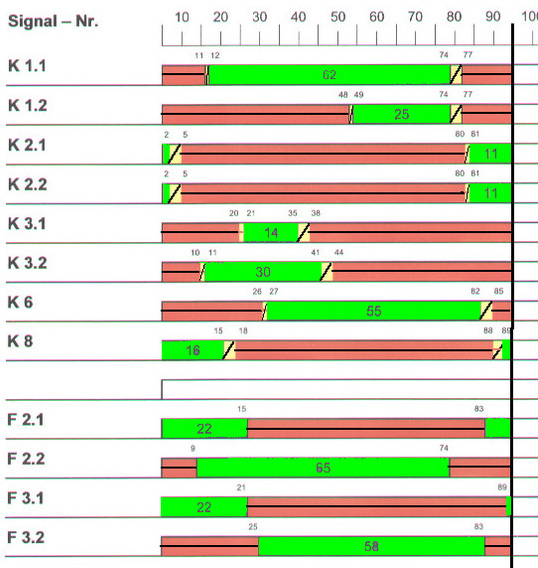
\includegraphics[width=0.7\textwidth]{signalzeitenplan_ausschnitt}
    \caption{Signalzeitenplan}
    \label{fig:signalzeitenplan}
\end{figure}

Auf der X-Achse befindet sich die Zeit in Sekunden, auf der Y-Achse die diskreten Werte der beteiligen Signalgeber. Rot- und Grünphasen sind in der jeweiligen Farbe dargestellt. Die übrigen Elemente entsprechen den beiden Gelbphasen Gelb und Rot/Gelb. Zu verstehen ist das Diagramm im Zeitfluss von links nach rechts. Rechts angekommen, geht es links wieder los.

Bei der verkehrsabhängigen Steuerung werden die einzelnen Verkehrsströme je nach Bedarf bedient. Sie funktioniert mithilfe vielerlei Technologien, so gibt es Induktionsschleifen und Bewegungsmelder, aber auch Videokameras unterstützen die Optimierung des Verkehrsflusses bei manchen Systemen. Vorwiegend handelt es sich dabei um Systeme, die an einzelnen Kreuzungen wirken und keinen größeren Bereich in Betracht ziehen. Sie sind zum Beispiel so konstruiert, dass alle ankommenden Fahrzeuge einer ankommenden Fahrzeugwelle die Kreuzung passieren können, die Ampelphasen werden dementsprechend angepasst. Dabei ist darauf zu achten, dass die Wartezeiten der anderen Verkehrsteilnehmer nicht unzumutbar werden oder ein Rückstau der Abbiegespuren entsteht, die die anderen Spuren einengt.

\begin{figure}[H]
    \centering
    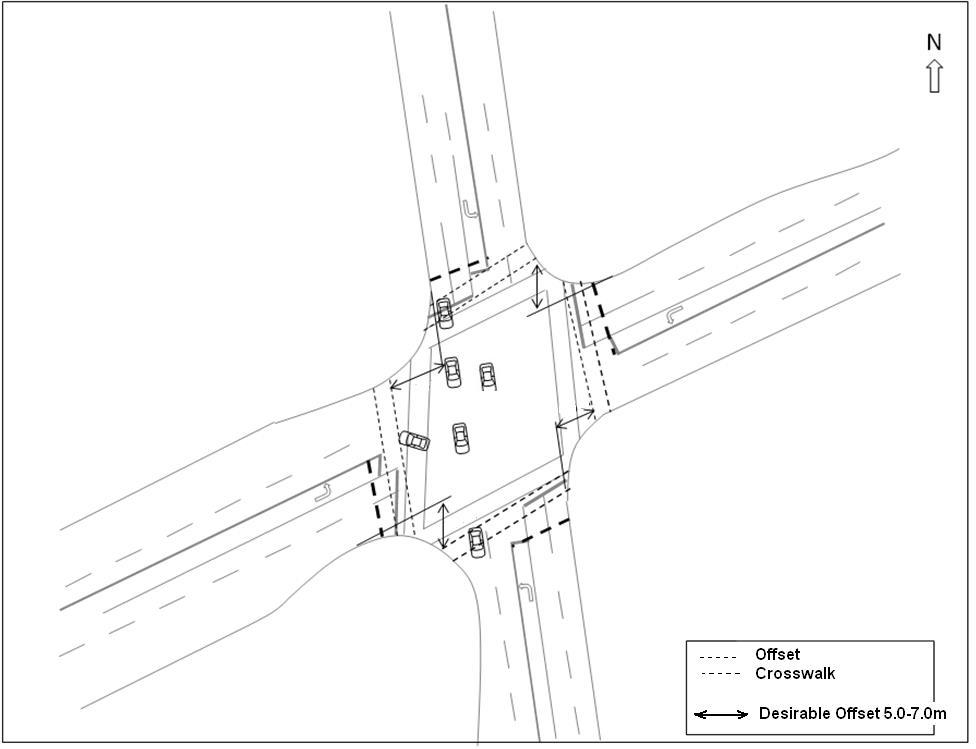
\includegraphics[width=0.7\textwidth]{offsetcrosswalk}
    \caption{Rückstau an einer Kreuzung}
    \label{fig:rueckstau}
\end{figure}

Daraus ergibt sich eine variable Umlaufzeit der Ampelphasen. Fest definierte Abläufe können zudem per Automatik zwischen verschiedenen Programmen wechseln, so kann auf verschiedene Verkehrsbelastungen (Berufs-, Tages- und Nachtverkehr usw.) reagiert werden.

Weitere Elemente des Straßenverkehrs, die den Verkehrsfluss direkt beeinflussen können, sind zum Beipiel Fußgängerampeln mit Anforderung oder einem Zebrastreifen. Es ist zwar wichtig, möchte man ein ganzheitliches System implementieren, diese Elemente zu betrachten, in dieser Ausarbeitung werden diese Elemente jedoch noch außen vorgelassen.

Der im Folgenden vorgestellte Optimierungsansatz mit dem Hopefield-Netzwerk betrachtet hingegen ein komplexes System an Straßen. Sozusagen einen Teilgraph des Verkehrsnetzes. Angewandt wurde das System im Zuge der Olympischen Spiele in Atlanta 1996\footnote{John F. G. and Khalid J. E., \href{https://www.aaai.org/Papers/Workshops/1993/WS-93-04/WS93-04-012.pdf}{Traffic Management Applications of Neural Networks,} \\https://www.aaai.org/Papers/Workshops/1993/WS-93-04/WS93-04-012.pdf}.

NOTES:
umlaufszeit 45 - 120 sek, Situation in HH
smart city 
atms
atlanta olympic
anforderung/bedarfsampeln

%\footnote{###NAME###, \href{###URL###}{###TITLE###,} \\###URL###}

\newpage

